% !TeX root = ../../thesis.tex
\chapter{Introduction}\label{ch:introduction}

%\instructionsintroduction

% Some dummy code to make sure bibtex does not complain.
\section{Electronic Processes in Biological Systems}

Electrons are at the heart of all biochemical processes. From the generation of energy to the synthesis of biomolecules, the movement and distribution of electrons govern the reactivity and function of biological systems. Many key biological reactions are, at their core, charge transfer processes—redox reactions where electrons are transferred from one molecule to another. These reactions are often catalyzed by enzymes, which provide the appropriate environment to facilitate electron movement, stabilize intermediates, and control reaction kinetics with remarkable specificity and efficiency.

One of the most prominent examples of biological electron transfer is the respiratory chain in mitochondria. In this complex pathway, electrons derived from metabolic substrates are transferred through a series of protein complexes and mobile carriers, such as cytochromes and quinones, ultimately reducing molecular oxygen to water. In the process, a proton gradient is generated across the inner mitochondrial membrane, driving ATP synthesis via chemiosmotic coupling. Quinones, in particular, play a central role as redox-active cofactors that shuttle electrons and protons, and their ability to stabilize semiquinone and anionic states is essential to their function.

Another striking example is oxygenic photosynthesis, carried out by plants, algae, and cyanobacteria. Light energy is captured by pigment-protein complexes and used to drive electron transfer through the photosynthetic electron transport chain. This process begins with the photoexcitation of chlorophyll in photosystem II and ultimately leads to the reduction of NADP\textsuperscript{+} to NADPH, with the concomitant generation of oxygen from water. The light-induced charge separation and subsequent electron transfer involve multiple cofactors, including chlorophylls, pheophytins, plastoquinones, and iron-sulfur clusters.

A third biological process involving complex electron dynamics is nitrogen fixation, carried out by nitrogenase enzymes in certain bacteria and archaea. Nitrogenase catalyzes the reduction of atmospheric nitrogen (N\textsubscript{2}) to ammonia (NH\textsubscript{3}), a reaction that requires the delivery of multiple electrons and protons. The enzyme contains a unique metallocluster cofactor (the FeMo-cofactor) that acts as a redox-active site for electron accumulation and N\textsubscript{2} activation. The electron flow is tightly regulated and coupled to ATP hydrolysis, and the mechanistic details of electron transfer and substrate binding remain areas of active research.

These examples illustrate the importance of electrons not just as abstract entities in chemical equations but as physical particles whose location, energy, and interactions must be understood to grasp biological function. Moreover, the existence of short-lived or weakly bound electronic states—such as nonvalence anions—can influence the dynamics of charge transfer processes, radical formation, and enzymatic activity. Understanding these transient electronic states requires experimental and computational tools capable of resolving both structure and electronic behavior on ultrafast timescales.

\subsection{Experimental Approaches for Characterizing Electron Transfer}

Studying such intricate electron-driven processes in biological systems is a challenging task that requires the integration of various experimental techniques. Traditionally, much of our understanding of enzymatic structure and function has come from structural biology. Techniques such as X-ray crystallography, nuclear magnetic resonance (NMR) spectroscopy, and cryo-electron microscopy (cryo-EM) allow researchers to determine the three-dimensional structures of proteins and complexes at atomic resolution. These structures are often deposited in public databases such as the Protein Data Bank (PDB), which provide critical starting points for further analysis.

Beyond static structures, insights into reaction mechanisms and kinetics are obtained through various spectroscopic methods. Ultraviolet-visible (UV-Vis) and infrared (IR) spectroscopy monitor changes in chromophores or functional groups during a reaction, while electron paramagnetic resonance (EPR) and Mössbauer spectroscopy provide information about unpaired electrons and metal centers. Time-resolved spectroscopy, including pump-probe and transient absorption techniques, captures short-lived intermediates in electron transfer processes, revealing their lifetimes and dynamics.

Mass spectrometry has also become a powerful tool in the analysis of biomolecular reactions. It can be used to identify reaction products, post-translational modifications, or radical intermediates with high sensitivity. However, while these experimental approaches provide indispensable data, they often capture only fragments of the complete picture. For example, spectroscopy may detect the presence of a transient intermediate without resolving its precise structure or the detailed path of electron movement between donor and acceptor. Similarly, crystallographic data can sometimes miss critical information—such as the position of hydrogen atoms, associated water networks, or dynamic conformational states—that is essential for understanding electron transfer.

\subsection{Modeling myBiological Electron Dynamics}

Given the limitations of experimental techniques in capturing the full complexity of electron transfer in biology, computational modeling has become an indispensable tool. Starting from experimentally resolved structures from the PDB, researchers apply various theoretical methods to simulate and predict biological behavior across multiple scales.

At the macroscopic level, coarse-grained models and network-based approaches can describe signaling pathways, metabolic fluxes, or cellular dynamics. On the molecular scale, molecular dynamics (MD) simulations are widely used to explore the conformational flexibility of proteins and nucleic acids over time. MD simulations model atoms as classical particles interacting via empirical force fields, allowing the exploration of structural fluctuations, binding events, and diffusion processes. Such simulations provide valuable insight into the dynamic context within which electron transfer occurs.

Recent advances in machine learning have had a profound impact on structural biology. Tools like AlphaFold have dramatically improved our ability to predict protein structures directly from amino acid sequences. Although these models rely on statistical learning methods rather than directly solving physical equations, they generate highly accurate structures that serve as vital starting points for further investigations into electronic properties.

To directly study electron transfer and electron dynamics, quantum mechanical (QM) methods are required. Approaches such as Hartree–Fock theory, density functional theory (DFT), and post-Hartree–Fock methods (e.g., coupled-cluster theory) solve or approximate solutions to the Schrödinger equation, treating electrons explicitly. These techniques reveal detailed information about chemical bonding, charge distribution, and reaction energetics. Despite their high accuracy, the computational cost of QM methods restricts their use to relatively small regions of a larger biological system, such as an enzyme active site or a cofactor.

Hybrid methods, notably quantum mechanics/molecular mechanics (QM/MM) simulations, provide a balance between accuracy and computational feasibility. In these methods, the region of primary interest—where electron transfer occurs—is treated using QM, while the surrounding environment is modeled using classical force fields. This allows a more realistic description of enzymatic reactions, electron transfer events, and proton-coupled mechanisms.

For elusive phenomena like nonvalence anionic states, even more sophisticated methods may be required. Such states, often weakly bound and highly sensitive to the surrounding electrostatic environment, may need advanced techniques that can capture long-range electron correlation and diffuse orbital characteristics. Methods such as equation-of-motion coupled-cluster theory (EOM-CC), Green's function approaches, and electron scattering calculations are sometimes employed to provide accurate descriptions of these transient states. Although these approaches come with significant computational cost, they are essential for uncovering the subtle electronic behavior that underpins key biological functions.

In summary, the integration of multiple modeling techniques—from coarse-grained methods to high-accuracy quantum approaches—enables a multiscale understanding of electron dynamics in biology. This holistic computational framework is crucial for elucidating the mechanisms of electron transfer and the roles played by nonvalence anions in biological systems, ultimately contributing to the broader understanding of enzymatic activity and energy conversion in living organisms.

Molecular anions are species in which a molecule possesses an extra electron, resulting in a negative charge. These systems are pervasive both in the gas phase and in biological environments. In many cases, molecular anions exhibit unusual stability, often persisting on timescales long enough to be isolated or characterized spectroscopically. Nonetheless, they are frequently transient intermediates, acting as precursors or doorway states that lead to further chemical transformations. Their behavior is intricately connected to factors such as molecular geometry, the environment (e.g., solvation or crystal lattice effects), and the energetic characteristics of the extra electron.

\section{Molecular Anions and Their Role in Chemical Processes}

The existence and behavior of molecular anions have been subjects of intense research because they encapsulate the interaction of excess electrons with molecular frameworks. In the gas phase, where perturbations from the environment are minimized, detailed studies have revealed long-lived anionic states that provide insight into intrinsic electron binding energies and the relaxation pathways following electron attachment. In contrast, within biological systems, the local environment, including solvent molecules and protein matrices, plays a significant role in stabilizing or destabilizing these excess electrons. This stabilization can lead to altered reactivities and modified pathways for both electron capture and subsequent chemical reactions.

\subsection{Nonvalence Anions: Diffuse Electronic States and Electron Capture}

Nonvalence anions represent a class of molecular anions where the extra electron occupies a diffuse orbital that is spatially decoupled from the usual valence orbitals of the molecule. This field, which emerged prominently among quantum chemists in the 1970s, has significantly advanced our understanding of electron localization in weak binding regimes.

\subsubsection{Characteristics and Formation}

In nonvalence anions, the additional electron is loosely attached, often residing in a highly diffuse orbital that extends well beyond the molecular skeleton. This leads to unique electronic states that differ markedly from those derived from traditional valence shell configurations. Because of the weak binding, nonvalence anions are extremely sensitive to external electric fields and the dielectric properties of their surroundings. 

\subsubsection{Role as Doorway States}

One of the most exciting aspects of nonvalence anions is their role as doorway states for electron capture processes. In many reactions, particularly those involving biological macromolecules, these states can serve as transient intermediates that facilitate the capture and eventual stabilization of electrons. An exemplar of this behavior is the solvated electron in water, where a nearly free electron is stabilized by a network of polar molecules. The interplay between nonvalence and valence electronic states in these systems can significantly influence reaction pathways and energy transfer processes.

\subsection{Dipole Anions: Formation, Stability, and Experimental Debate}

Dipole-bound anions are a subset of molecular anions that rely on the permanent dipole moment of a molecule for electron stabilization. When a molecule exhibits a sufficiently large dipole moment—typically exceeding a critical threshold that depends on the molecular structure and polarizability—the electrostatic potential can capture an excess electron in a diffuse orbital\cite{jordan2003theory}.

\subsubsection{Critical Dipole Moment and Formation Criteria}

The formation of a dipole-bound anion depends critically on the magnitude of the molecular dipole moment. Theoretical models predict that once the dipole moment surpasses a certain critical value (generally in the range of 2.5 to 2.8 Debye), the electron is capable of being bound in a diffuse orbital. Experimental investigations in the gas phase have confirmed the formation of dipole-bound states for a variety of molecules, revealing subtle dependencies on molecular geometry and polarizability.

\subsubsection{Stability and Relevance in Different Phases}

Despite their apparent stability in isolated gas-phase experiments, dipole-bound anions are often very short-lived species. Their transient nature arises due to the weak binding energy of the extra electron, making these states highly susceptible to perturbations such as collisions or solvation effects. While extensive studies have been conducted in the gas phase, the existence and stability of dipole-bound anions in solvated or biological environments remain topics of ongoing debate. In polar solvents, the competition between solvation stabilization and charge delocalization leads to complex behavior, and the experimental evidence for dipole-bound states in such systems is not always consistent.

\subsection{Conclusion}

In summary, molecular anions—encompassing both nonvalence and dipole-bound varieties—serve as key intermediates and transient states in a range of chemical and biological processes. Their unique electronic structures and sensitivities to their environments not only challenge our understanding of electron-molecule interactions but also provide critical insights into the mechanisms underlying electron capture and transfer. Continuing research in this field is essential for advancing our knowledge of fundamental chemical processes, with implications spanning from atmospheric chemistry to biological electron transfer and beyond.



\section{Electrons in Biology}
\ldots
Explain reactions in biology, charge transfer reaction... Electrons are essential. Most reactions are conducted by enzymes... Some importnat pathways as respiratory chain (mention quinones), photosinthesis, nitrogenase...
\subsection{How do We Get Knowledge About these systems?}
How do we study enzymes... Protein crystalography, NMR etc... Structures are stored in the PDB... Can study by kinetics reactions by spectroscopy, mass spectroscopy... But experimental methods cannot ptovide the complete picture by themselves\dots

\subsection{How do we model biology}
Starting from the structures from the PDB, meny methods have been developed MD, AI (AlphaFold), QM... Each method seerves to provide a different view of the problem (kynetics, structure, thermodynamics...). Each method treats a different scale at different costs and accuracies... To model electron and electron dynamics we need high accuracy and costly methods...

\section{Molecular Anions}
Explain what is a molecular anion, how they exist in gas phase and in biology. They long lived times. They are usually transient species in time leading to other products.
\ldots
\subsection{Nonvalence Anions}
A field developed by quantum chemists from the 70s, the electron resides in a diffuse orbital. They are low energy lying stes that are very interesting when convined with a valence anion stat. They can act as doorway state to electron capture... Types of nonvalence anions. Examples of importnat systems as the solvated electron in water.
\ldots
\subsection{Dipole Anions}
\ldots
Explain dipole bond anions. Critical dipole moments, again explain they are shortlived species. They have been studied in the gas phase extensively and there is debate on their existance in solvated systems.
\section{Do Non-valence Anions Play a Critical Role in Biology?}
Extensive wotk related to radiation damaga to the DNA as well as investigation on radiosesitizers... However little has been done in trying to asses their role in natural pathways. They could provide an elegant way to regulate long range electron transfer.
A reason for its little investigation is the high cost of the needed methods to study them (CCSD, CASSCF...), and the little overlap between the research fields of the fields involved... This work aims to bridge this gap... 
\ldots
\subsection{Biological Quinones}
Quinones are a class of molecules that are everywhere in biology... they are essential to electron transfer pathways such as the respitatory chain and photosinthesis., They act as electron carriers between different enzimes... Coenzyme Q is one of the most common quinone... It presents a very interesting structure to study the role of nonvalence anions as it suports both a valence anion and dipole anion... It is possible that these states are not useful as they are very widespread but we want to asses the feasibility of their existance... 
\ldots

\section{Remove from here on}

% Some dummy code show how to include images.
\begin{figure}[th!]
  \centering
  \medskip
  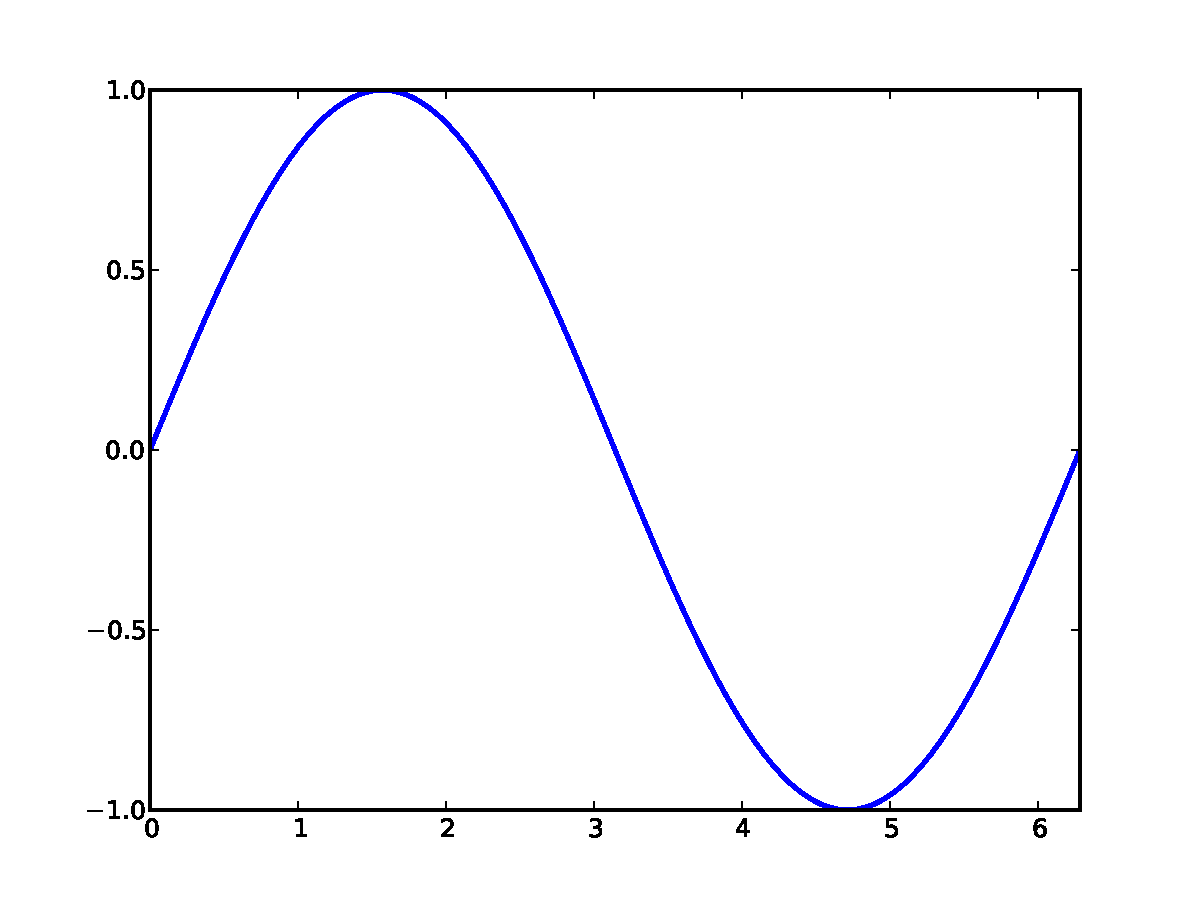
\includegraphics[width=.9\textwidth]{sine}
  \caption[Short caption for Table of Figures]{Illustration of how to
  include a figure (long text, should not go to Table of Figures).}
  \label{fig:sine}
\end{figure}

%Add list of symbols and abbreiations here:
% Some dummy code to get at least 1 entry in the nomenclature.
\nomenclature{$\Theta$}{A nice symbol}
Introducing some symbol: $\Theta$.

% Some dummy code to get at least 1 entry in the list of
% abbreviations.
\newglossaryentry{md}{name={MD},description={molecular dynamics}}
Introducing an acronym: \gls{md}.

\begin{figure}[th!]
  \centering
  % GNUPLOT: LaTeX picture with Postscript
\begingroup
  \makeatletter
  \providecommand\color[2][]{%
    \GenericError{(gnuplot) \space\space\space\@spaces}{%
      Package color not loaded in conjunction with
      terminal option `colourtext'%
    }{See the gnuplot documentation for explanation.%
    }{Either use 'blacktext' in gnuplot or load the package
      color.sty in LaTeX.}%
    \renewcommand\color[2][]{}%
  }%
  \providecommand\includegraphics[2][]{%
    \GenericError{(gnuplot) \space\space\space\@spaces}{%
      Package graphicx or graphics not loaded%
    }{See the gnuplot documentation for explanation.%
    }{The gnuplot epslatex terminal needs graphicx.sty or graphics.sty.}%
    \renewcommand\includegraphics[2][]{}%
  }%
  \providecommand\rotatebox[2]{#2}%
  \@ifundefined{ifGPcolor}{%
    \newif\ifGPcolor
    \GPcolortrue
  }{}%
  \@ifundefined{ifGPblacktext}{%
    \newif\ifGPblacktext
    \GPblacktexttrue
  }{}%
  % define a \g@addto@macro without @ in the name:
  \let\gplgaddtomacro\g@addto@macro
  % define empty templates for all commands taking text:
  \gdef\gplbacktext{}%
  \gdef\gplfronttext{}%
  \makeatother
  \ifGPblacktext
    % no textcolor at all
    \def\colorrgb#1{}%
    \def\colorgray#1{}%
  \else
    % gray or color?
    \ifGPcolor
      \def\colorrgb#1{\color[rgb]{#1}}%
      \def\colorgray#1{\color[gray]{#1}}%
      \expandafter\def\csname LTw\endcsname{\color{white}}%
      \expandafter\def\csname LTb\endcsname{\color{black}}%
      \expandafter\def\csname LTa\endcsname{\color{black}}%
      \expandafter\def\csname LT0\endcsname{\color[rgb]{1,0,0}}%
      \expandafter\def\csname LT1\endcsname{\color[rgb]{0,1,0}}%
      \expandafter\def\csname LT2\endcsname{\color[rgb]{0,0,1}}%
      \expandafter\def\csname LT3\endcsname{\color[rgb]{1,0,1}}%
      \expandafter\def\csname LT4\endcsname{\color[rgb]{0,1,1}}%
      \expandafter\def\csname LT5\endcsname{\color[rgb]{1,1,0}}%
      \expandafter\def\csname LT6\endcsname{\color[rgb]{0,0,0}}%
      \expandafter\def\csname LT7\endcsname{\color[rgb]{1,0.3,0}}%
      \expandafter\def\csname LT8\endcsname{\color[rgb]{0.5,0.5,0.5}}%
    \else
      % gray
      \def\colorrgb#1{\color{black}}%
      \def\colorgray#1{\color[gray]{#1}}%
      \expandafter\def\csname LTw\endcsname{\color{white}}%
      \expandafter\def\csname LTb\endcsname{\color{black}}%
      \expandafter\def\csname LTa\endcsname{\color{black}}%
      \expandafter\def\csname LT0\endcsname{\color{black}}%
      \expandafter\def\csname LT1\endcsname{\color{black}}%
      \expandafter\def\csname LT2\endcsname{\color{black}}%
      \expandafter\def\csname LT3\endcsname{\color{black}}%
      \expandafter\def\csname LT4\endcsname{\color{black}}%
      \expandafter\def\csname LT5\endcsname{\color{black}}%
      \expandafter\def\csname LT6\endcsname{\color{black}}%
      \expandafter\def\csname LT7\endcsname{\color{black}}%
      \expandafter\def\csname LT8\endcsname{\color{black}}%
    \fi
  \fi
    \setlength{\unitlength}{0.0500bp}%
    \ifx\gptboxheight\undefined%
      \newlength{\gptboxheight}%
      \newlength{\gptboxwidth}%
      \newsavebox{\gptboxtext}%
    \fi%
    \setlength{\fboxrule}{0.5pt}%
    \setlength{\fboxsep}{1pt}%
    \definecolor{tbcol}{rgb}{1,1,1}%
\begin{picture}(4600.00,4320.00)%
    \gplgaddtomacro\gplbacktext{%
      \csname LTb\endcsname%%
      \put(714,562){\makebox(0,0)[r]{\strut{}$-1.5$}}%
      \csname LTb\endcsname%%
      \put(714,1156){\makebox(0,0)[r]{\strut{}$-1$}}%
      \csname LTb\endcsname%%
      \put(714,1749){\makebox(0,0)[r]{\strut{}$-0.5$}}%
      \csname LTb\endcsname%%
      \put(714,2343){\makebox(0,0)[r]{\strut{}$0$}}%
      \csname LTb\endcsname%%
      \put(714,2936){\makebox(0,0)[r]{\strut{}$0.5$}}%
      \csname LTb\endcsname%%
      \put(714,3530){\makebox(0,0)[r]{\strut{}$1$}}%
      \csname LTb\endcsname%%
      \put(714,4124){\makebox(0,0)[r]{\strut{}$1.5$}}%
      \csname LTb\endcsname%%
      \put(812,386){\makebox(0,0){\strut{}$-10$}}%
      \csname LTb\endcsname%%
      \put(1680,386){\makebox(0,0){\strut{}$-5$}}%
      \csname LTb\endcsname%%
      \put(2549,386){\makebox(0,0){\strut{}$0$}}%
      \csname LTb\endcsname%%
      \put(3417,386){\makebox(0,0){\strut{}$5$}}%
      \csname LTb\endcsname%%
      \put(4286,386){\makebox(0,0){\strut{}$10$}}%
    }%
    \gplgaddtomacro\gplfronttext{%
      \csname LTb\endcsname%%
      \put(3530,3965){\makebox(0,0)[r]{\strut{}$\sin(x)$}}%
      \csname LTb\endcsname%%
      \put(3530,3789){\makebox(0,0)[r]{\strut{}$\cos(x)$}}%
      \csname LTb\endcsname%%
      \put(3530,3613){\makebox(0,0)[r]{\strut{}$\tan(x)$}}%
      \csname LTb\endcsname%%
      \put(161,2343){\rotatebox{-270.00}{\makebox(0,0){\strut{}$y$}}}%
      \csname LTb\endcsname%%
      \put(2549,123){\makebox(0,0){\strut{}$x$}}%
    }%
    \gplbacktext
    \put(0,0){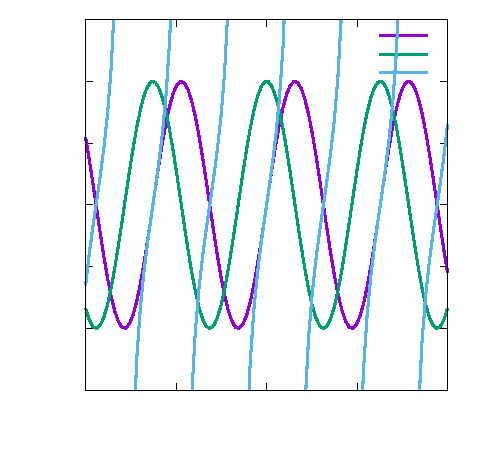
\includegraphics[width={230.00bp},height={216.00bp}]{test}}%
    \gplfronttext
  \end{picture}%
\endgroup

  %figsize is set in image/test.gp 
  \caption[Short caption for Table of Figures]{Illustration of how to
  include a figure (long text, should not go to Table of Figures).}
  \label{fig:test}
\end{figure}

%%%%%%%%%%%%%%%%%%%%%%%%%%%%%%%%%%%%%%%%%%%%%%%%%%
% Keep the following \cleardoublepage at the end of this file, 
% otherwise \includeonly includes empty pages.
\cleardoublepage

% vim: tw=70 nocindent expandtab foldmethod=marker foldmarker={{{}{,}{}}}
